% Search for all the places that say "PUT SOMETHING HERE".

\documentclass[11pt]{article}
\usepackage{amsmath,textcomp,amssymb,geometry,graphicx,enumerate}
\usepackage{ctex}

\def\Name{了然}  % Your name
\def\SID{2016302580055}  % Your student ID number
\def\Homework{3} % Number of Homework
\def\Session{Spring 2019}


\title{\Large Networks and Distributed Computing --- Spring 2019 --- Homework \Homework\ }
\author{\Name, Student ID: \SID}
\markboth{Networks and Distributed Computing--\Session\  Homework \Homework\ \Name}{Networks and Distributed Computing--\Session\ Homework \Homework\ \Name}
\pagestyle{myheadings}
\date{\today}

\newenvironment{qparts}{\begin{enumerate}[{(}a{)}]}{\end{enumerate}}
\def\endproofmark{$\Box$}
\newenvironment{proof}{\par{\bf Proof}:}{\endproofmark\smallskip}

\textheight=9in
\textwidth=6.5in
\topmargin=-.75in
\oddsidemargin=0.25in
\evensidemargin=0.25in


\begin{document}
\maketitle

\section{TCP Demo Program}

\begin{figure}[h]
\centering
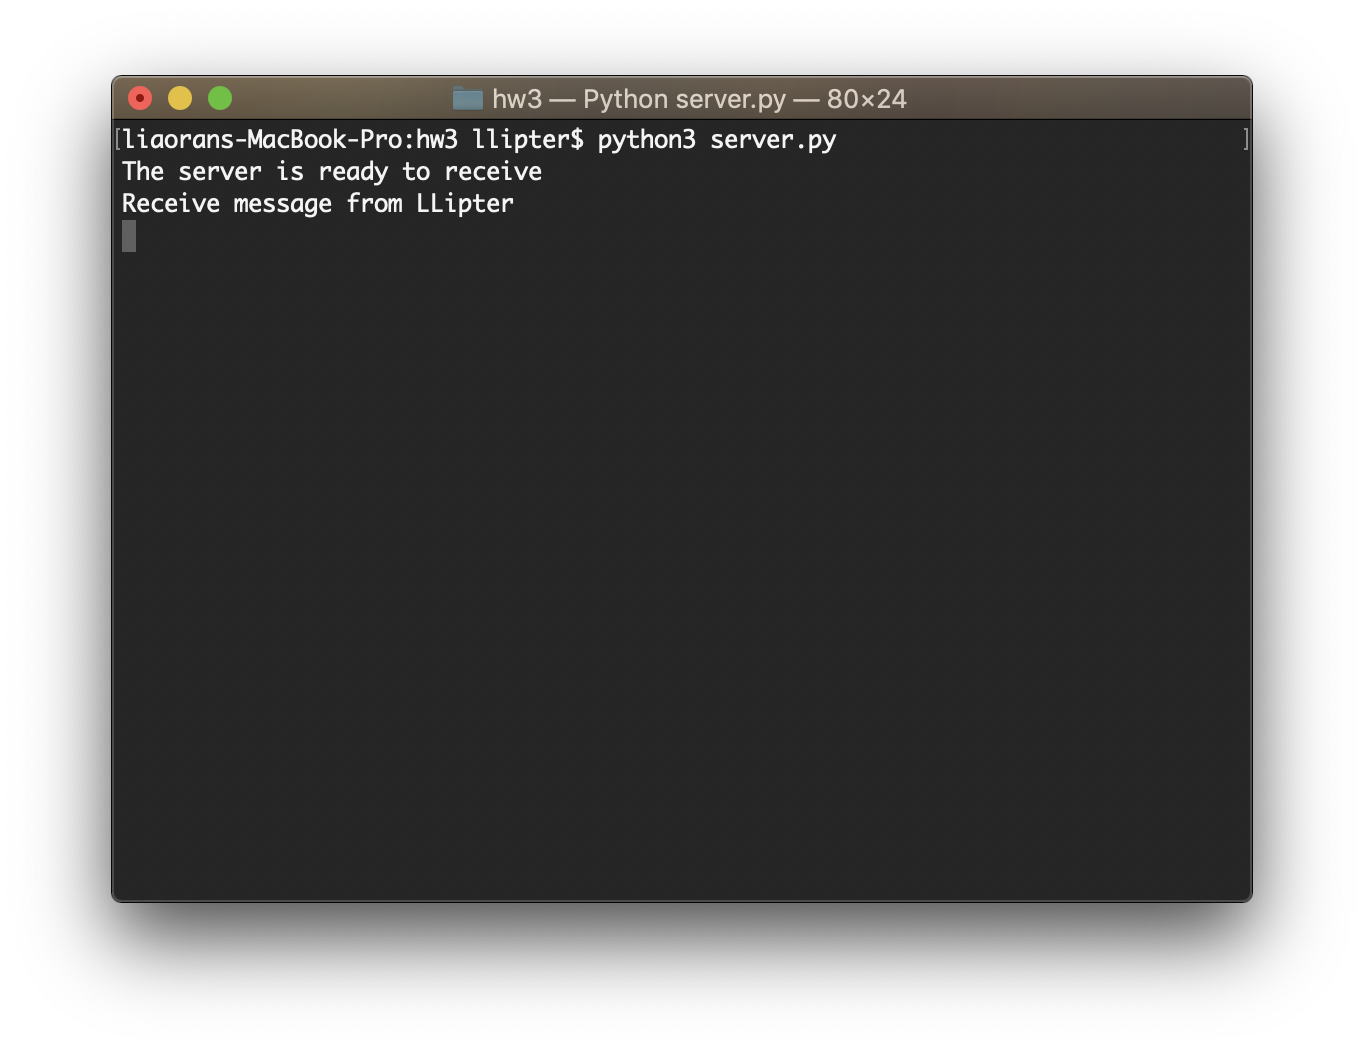
\includegraphics[width=.5\textwidth]{server.png}
\caption{\label{fig:server}server.py}
\end{figure}

\begin{figure}[h]
\centering
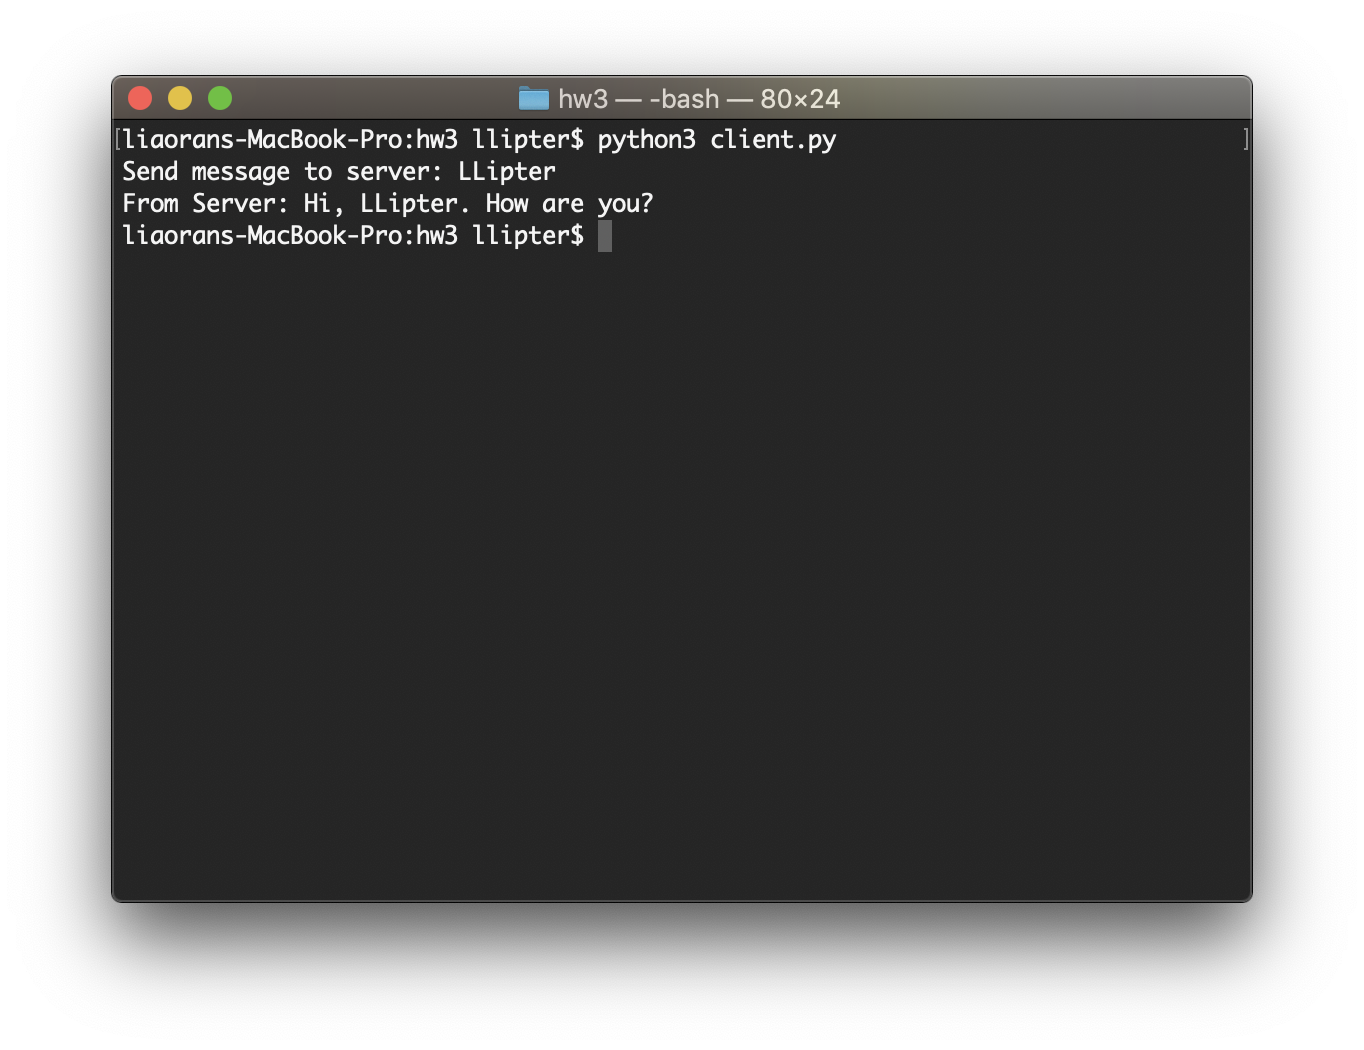
\includegraphics[width=.5\textwidth]{client.png}
\caption{\label{fig:client}client.py}
\end{figure}

\newpage
\section{Problem 1}

\textbf{Suppose Client A requests a web page from Server S through HTTP and its socket is associated with port 33000.}

\begin{qparts}

	\item \textbf{What are the source and destination ports for the segments sent from A to S?}
	
	Source port is 33000 and destination port is 80.
	
	\item \textbf{What are the source and destination ports for the segments sent from S to A?}

	Source port is 80 and destination port is 33000.
	
	\item \textbf{Can Client A contact to Server S using UDP as the transport protocol?}
	
	No. HTTP is built upon TCP.
	
	\item \textbf{Can Client A request multiple resources in a single TCP connection}
	
	Yes. there's no limit on how many data can be transported through a single TCP connection.

\end{qparts}


\newpage
\section{Problem 2}

\textbf{Consider Figure 3.5. What are the source and destination port values in the seg- ments flowing from the server back to the clients’ processes? What are the IP addresses in the network-layer datagrams carrying the transport-layer segments?}

~\\

Suppose the IP addresses of the hosts $A, B$, and $C$ are $a, b, c$, respectively. 

To host $A$: Source port = 80, source IP address = $b$, dest port = 26145, dest IP address = $a$.

To host $C$, left process: Source port = 80, source IP address = $b$, dest port = 7532, dest IP address = $c$.

To host $C$, right process: Source port = 80, source IP address = $b$, dest port = 26145, dest IP address = $c$.


\newpage
\section{Problem 4}

\textbf{Assume that a host receives a UDP segment with 01011101 11110010 (we separated the values of each byte with a space for clarity) as the checksum. The host adds the 16-bit words over all necessary fields excluding the checksum and obtains the value 00110010 00001101. Is the segment considered correctly received or not? What does the receiver do?}

~\\

 
\begin{center} 
\begin{tabular}{ccccccccccccccccccc}
	&  & 0&1&0&1&1&1&0&1 & &1&1&1&1&0&0&1&0 \\
	&+& 0&0&1&1&0&0&1&0 & &0&0&0&0&1&1&0&1 \\
	\hline
	&  & 1&0&0&0&1&1&1&1 & &1&1&1&1&1&1&1&1 \\
\end{tabular}
\end{center}

As demonstrated above, the overall checksum contains 0. Therefore, it is not valid. The receiver will drop this packet and wait for retransmitting.




\newpage
\section{Problem 28}

\textbf{Host A and B are directly connected with a 100 Mbps link. There is one TCP connection between the two hosts, and Host A is sending to Host B an enormous file over this connection. Host A can send its application data into its TCP socket at a rate as high as 120 Mbps but Host B can read out of its TCP receive buffer at a maximum rate of 50 Mbps. Describe the effect of TCP flow control.}

~\\

Since the link capacity is only 100 Mbps, so host A’s sending rate can be at most 100Mbps. Still, host A sends data into the receive buffer faster than Host B can remove data from the buffer. The receive buffer fills up at a rate of roughly 50Mbps. When the buffer is full, Host B signals to Host A to stop sending data by setting $RcvWindow = 0$. Host A then stops sending until it receives a TCP segment with $RcvWindow > 0$. Host A will thus repeatedly stop and start sending as a function of the $RcvWindow$ values it receives from Host B. On average, the long-term rate at which Host A sends data to Host B as part of this connection is no more than 50Mbps.


\newpage
\section{Problem 40}

\textbf{Consider Figure 3.58. Assuming TCP Reno is the protocol experiencing the behavior shown above, answer the following questions. In all cases, you should provide a short discussion justifying your answer.}

\begin{qparts}
	\item \textbf{Identify the intervals of time when TCP slow start is operating.}

	TCP slowstart is operating in the intervals [1,6] and [23,26]
	
	\item \textbf{Identify the intervals of time when TCP congestion avoidance is operating.}
	
	TCP congestion avoidance is operating in the intervals [6,16] and [17,22]
	
	\item \textbf{After the 16th transmission round, is segment loss detected by a triple duplicate ACK or by a timeout?}
	
	 After the 16th transmission round, packet loss is recognized by a triple duplicate ACK. If there was a timeout, the congestion window size would have dropped to 1.
	
	\item \textbf{After the 22nd transmission round, is segment loss detected by a triple duplicate ACK or by a timeout?}
	
	After the 22nd transmission round, segment loss is detected due to timeout, and hence the congestion window size is set to 1.
	
\end{qparts}

\end{document}